% % Created 2015-09-15 Tue 11:46
% \documentclass[11pt]{article}
% \usepackage[utf8]{inputenc}
% \usepackage[T1]{fontenc}
% \usepackage{fixltx2e}
% \usepackage{graphicx}
% \usepackage{longtable}
% \usepackage{float}
% \usepackage{wrapfig}
% \usepackage{rotating}
% \usepackage[normalem]{ulem}
% \usepackage{amsmath}
% \usepackage{textcomp}
% \usepackage{marvosym}
% \usepackage{wasysym}
% \usepackage{amssymb}
% \usepackage{hyperref}
% \usepackage{color}
% \usepackage{soul}
% \tolerance=1000
% \usepackage[margin=1in]{geometry}

% \newcommand{\hilight}[1]{\colorbox{yellow}{#1}}

% %\author{Alex Ansari}
% %\date{}
% %\title{TALOS}
% %\hypersetup{
% %  pdfkeywords={},
% %  pdfsubject={},
% %  pdfcreator={Emacs 24.3.1 (Org mode 8.2.10)}}


% \begin{document}
\section{RoboKnee}
\label{roboKnee}
\begin{refsection}[exos/roboKnee.bib]


The RoboKnee is a prototype system designed to enhance human strength, endurance and speed.  To achieve these goals, RoboKnee uses a low-impedance mechanical system that incorporates a natural user interface, long life, and is comfortable to wear.  The suit's controller implements a ``get out of the way'' control scheme, where the system interacts with the user through a low-impedance interface.  This section focuses on RoboKnee's linear series elastic actuator design and the novel control method the device employs to coordinate its single powered knee joint.

\subsection{Actuator specifications}

The RoboKnee actuator is specifically designed to provide low impedance and high force feedback fidelity.  The device uses a series elastic actuator to obtain robust output force measurements.  The series elastic actuation scheme allows RoboKnee to avoid load cells, which are both delicate and expensive.

The actuator used in the RoboKnee device (see Figure \ref{fig:roboAct}) consists of a drive train and output carriage. These two sub-assemblies are coupled through die compression springs.  A servo motor directly connected to a ball screw assembly drives a ball nut flange that pushes on a spring retaining plate.  A secondary spring retaining plate is coupled to an output assembly.  By measuring the deflection in the die springs, RoboKnee is able to obtain the force applied to the output of the linear SEA.  
\begin{figure}[thpb]
\centering
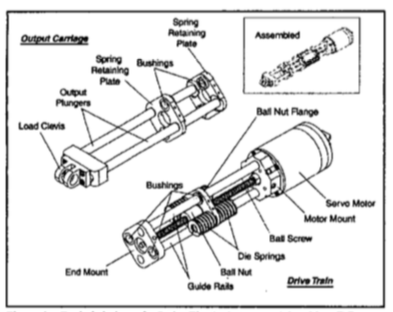
\includegraphics[width=3.in]{exos/figs/roboKnee/roboSEA}
  \caption{Exploded view of a series-elastic actuator.}
%  \vspace{-0.2in}
 \label{fig:roboAct}   
 \end{figure}

The linear actuator pictured in Figure \ref{fig:roboAct} { \bf weighs 1.13 kg, has a stroke length of 30.5 cm and diameter of 5.8 cm}.  The {\bf maximum speed of the actuator is 28 cm/s}.  The actuator's {\bf maximum continuous force is 565N and its maximum peak force is 1,330 N}, with a {\bf maximum continuous power of output of 164 W, and maximum peak power of 634 W}.   

The force control bandwidth of the RoboKnee actuator is dependent on the magnitude of the force.  Larger forces can induce significant time delays due to the time it takes for the spring to compress.  Thus, the {\bf small force control bandwidth of the system is 35 Hz} and the {\bf high force bandwidth is around 7.5 Hz}. 
 
 \subsection{Exoskeleton Specifications}
 
 The RoboKnee mechanism consists of a single actuated degree of freedom powering the flexion/extension of the operator's knee joint.  Note that the mechanism itself does not provide a pathway for transferring weight from a load directly to the ground.  The mechanism transfers loads directly to the users musculoskeletal structure, and focuses primarily on augmenting user knee joint torques.
 
 The RoboKnee device is composed of an off-the-shelf knee brace modified with structural pieces to extend the brace and provide actuator attachment points (see Figure~\ref{fig:roboKnee}).
 \begin{figure}[thpb]
\centering
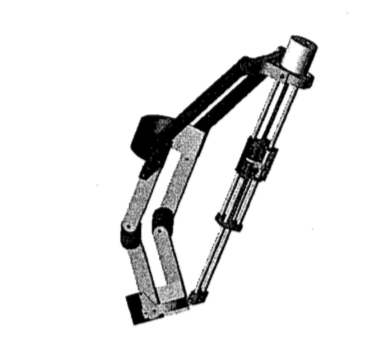
\includegraphics[width=3.in]{exos/figs/roboKnee/roboBrace}
  \caption{RoboKnee design.}
%  \vspace{-0.2in}
 \label{fig:roboKnee}   
 \end{figure}
 The exact length between actuator attachment points is not listed in the literature, but it appears as though the attachment points are at a minimum of one actuator stroke displacement away from each other. Thus, we assume a {\bf minimum moment arm of 30.5 cm} is a reasonable approximation.
 
 RoboKnee uses a \textbf{linear potentiometer} spanning the spring retaining plates to measure displacement in the springs and subsequently to measure force at the actuator output.  The forces between the users foot and the ground are also measured using \textbf{single axis load cells}.  Potentiometers which measure the knee joint angle are also employed in this design.     
 
 The single actuator as well as control and sensor electronics are run using {\bf 4 kg of nickel-metal-hydride batteries, which give the system only about 30-60 minutes of heavy use}.
 
 
 \subsection{Control Specifications}
 
 RoboKnee employs a hierarchical control strategy, which uses a straightforward mid-level force generation scheme coupled with a low-level closed-loop force-based control loop.  The low-level (joint level) control is a PD control loop.
 
 The RoboKnee's mid-level controller uses several simplifying assumptions to perform ``force amplification'' to offload a percentage of the torque required by the user to actuate the system's knee joint.  This is achieved through positive force feedback amplification.  The approach uses the measured ground reaction force to calculate the torque that would be required to produce this force in a static situation, \[ {\bf \tau} = \vR \times \vF.\]  The $\vR$ term represents the vector from the ground reaction force to the user's knee and $\vF$ is the ground reaction force.  Note that in RoboKnee's implementation, $\vF$ can only be estimated due to the fact that the ankle joint angle and the ground reaction force is assumed to be purely vertical (a limitation induced by the single axis force sensors on the user's feet).
   
   
 Once the estimated joint torque, ${\bf \tau}$, is calculated, an amplification factor specifies how much of the required knee torque will be provided by the control system.  For example, with unity amplification factor, the actuator would completely compensate for the sensed ground reaction forces.  Similarly, with zero amplification, the exoskeleton provides no force.
  
 
 \subsection{Assessment and Recommendations} 
 
 The RoboKnee is a relatively simple system that highlights several intelligent hardware and control design concepts.  The use of a linear ball screw with a series elastic element that enables high-fidelity force control is a very good idea. The idea of using the measured ground reaction forces to produce the desired knee joint torque is also interesting in the sense that it is very simple and relies on a minimal amount of information.
 
 The overall design of the RoboKnee mechanism is most likely not optimal, as it significantly increases the effective volume of the operator-system leg, but as a prototype, this concept offers interesting benefits.
 
 The discussion as well as figures in this section are respectively based on and taken from \cite{robo_knee_2004}.  
 
\printbibliography[heading=subbibliography]

\end{refsection}

 
 % \end{document}
 
 % Jerry E. Pratt and Benjamin T. Krupp and Christopher J. Morse and Steven Collins, "The RoboKnee: An Exosskeleton for Enhancing Strength and Endurance During Walking," International Conference on Robotics and Automation, 2004, pp. 2430-2435.
 
 
 
%%% Local Variables:
%%% mode: latex
%%% TeX-master: "../survey"
%%% End:
